\documentclass{beamer}

% Theme
%\usetheme{Madrid}
%\usecolortheme{default}
\mode<presentation>
{
  \usetheme{Warsaw}
  \setbeamercovered{transparent}
}

\usetheme{Warsaw}

\setbeamersize{text margin left=3mm}
\setbeamersize{text margin right=3mm}

% Packages
\usepackage[utf8]{inputenc}
\usepackage[backend=bibtex, style=authoryear]{biblatex} % You can change the style if you prefer a different citation style
\addbibresource{Chp1.bib}

\usepackage{dirtytalk}
\usepackage{cancel}
\usepackage{graphicx}
\usepackage{wrapfig}
\usepackage{caption}
\usepackage{booktabs}
\usepackage{adjustbox}
\usepackage{amssymb}
\usepackage{xcolor}



% Title slide
\title[]{Heterogeneous Returns and the Distribution of Wealth}
\author[Edwards]{Decory Edwards}
\institute[JHU]{Johns Hopkins University}
\date{\today}

\begin{document}

\begin{frame}
  \titlepage
\end{frame}

%%%%%%%%%%%%%%%%%%%%
\section{Introduction}

\begin{frame}{Brief history on wealth inequality}
  \cite{jbab18} offer a useful survey of lit

  \vspace{2.5mm}
\begin{enumerate}
\item Observable skewness in wealth holdings $\rightarrow$ assume distributional properties
\item Use distribution of income to explain distribution of wealth
\item Describe the dynamics of optimal consumption-saving behavior
\end{enumerate}

\vspace{2.5mm}
an interest in wealth inequality $\rightarrow$ heterogeneous agent macro modeling.

\end{frame}

%%%%%%%%%%%%%%%%%%%%%%%

\begin{frame}{Measured heterogeneity in returns}

 \begin{figure}
    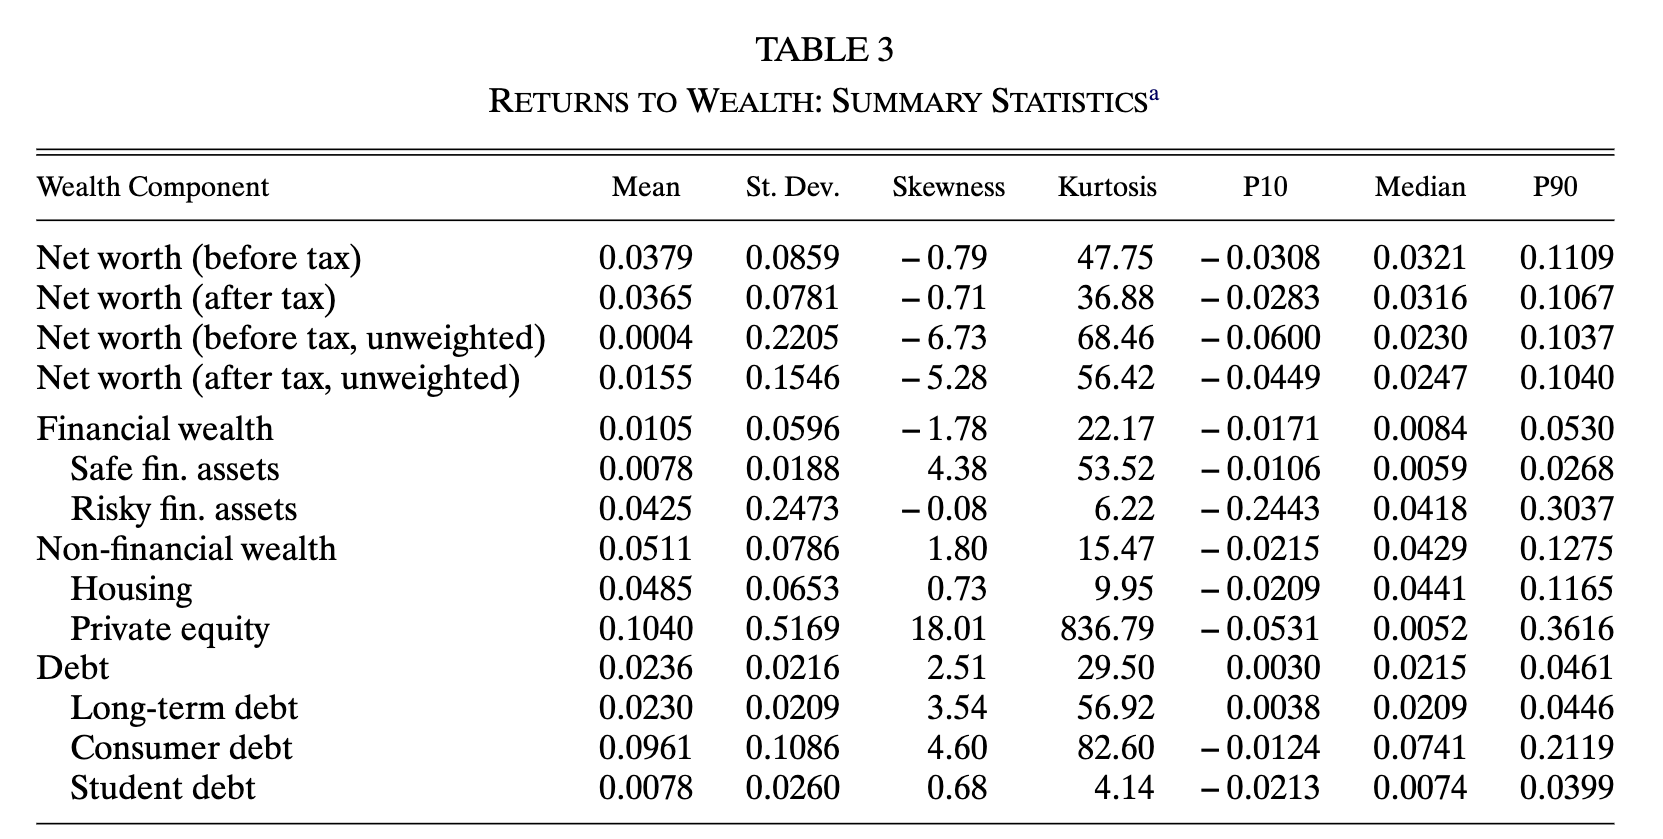
\includegraphics[height=.6\textheight]{Figures/Fagereng2020Tab3.png}
    \captionsetup{font=scriptsize}
    \caption{Distribution of returns in narrowly defined asset classes from \cite{aflgdmlp20}.}
  \end{figure}

 % \begin{itemize}
 % \item Technical: Savings grow across periods through the interest rate
 % \item Empirical: Returns are positively correlated with wealth
  %  \end{itemize}


\end{frame}
%%%%%%%%%%%%%%%%%%

\begin{frame}{Outline}
\begin{enumerate}
\item Empirical evidence of heterogeneous returns
\item Model
\item Structural estimation to match wealth data
\end{enumerate}

\vspace{2.5mm}
\textit{Life-cycle model with het. returns generates a reasonably skewned distribution.}


\end{frame}
%%%%%%%%%%%%%%%%%%

\begin{frame}{My contribution}


\begin{itemize}
  \item Why returns? $\rightarrow$ an observable feature of household's problem
\item Labor income process: Random walk v.s. AR$(1)$
\item Age-education dependent labor income process and mortality rates
\end{itemize}
\end{frame}
%%%%%%%%%%%%%%%%%%

\subsection{Heterogeneous Returns in the Data}
\begin{frame}{What are het. returns?}

   \begin{columns}
     \column{0.5\textwidth}
     \small
     From optimal portfolio choice theory...
    \centering

    \begin{itemize}
    \item Optimal share in the risky asset is
    $$ \alpha_{it}^{m} = \frac{\mathbb{E}(r_{t}^{m} - r_{t}^{s})}{\gamma_i \sigma^{2}_{t}}.$$
    \item Individual \textit{realized} return is
    $$ r_{it}^{f} = r_{t}^{s} + \alpha_{it}^{m} (r_{t}^{m} - r_{t}^{s}). $$
    \end{itemize}

    \column{0.5\textwidth}
    \centering
    \begin{figure}
    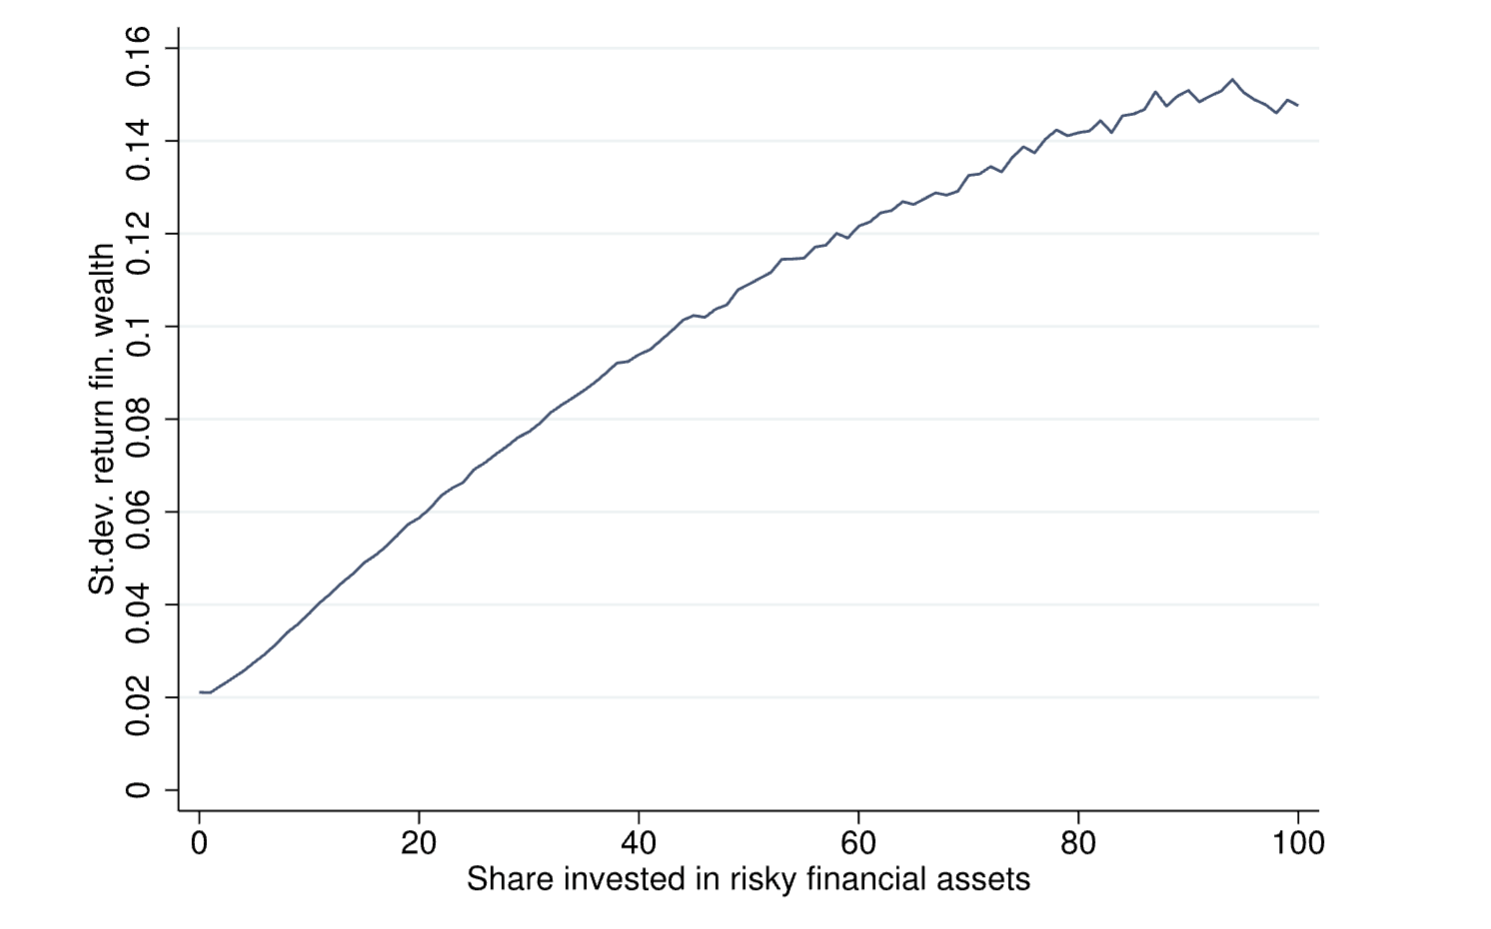
\includegraphics[width=\textwidth]{Figures/Fagereng2020Fig1.png}
    \captionsetup{font=scriptsize}
    \caption{Heterogeneity in returns to financial wealth by share of risky assets from \cite{aflgdmlp20}.}
    \end{figure}
  \end{columns}

\end{frame}
%%%%%%%%%%%%%%%%

\begin{frame}{Empirical estimate of heterogeneity}

     \begin{columns}
     \small
     \column{0.5\textwidth}
    \centering

    \begin{itemize}
    \item Step 1: panel regression on returns
    $$ r^{n}_{it} = X^{'}_{it} \beta + u_{it}. $$
    \item Step 2: Add fixed effects
    $$ u_{it} = f_{i} + e_{it}. $$
    $\implies R^2$ goes from $.33$ to $.5$.
    \end{itemize}


    \column{0.5\textwidth}
    \centering
    \begin{figure}
    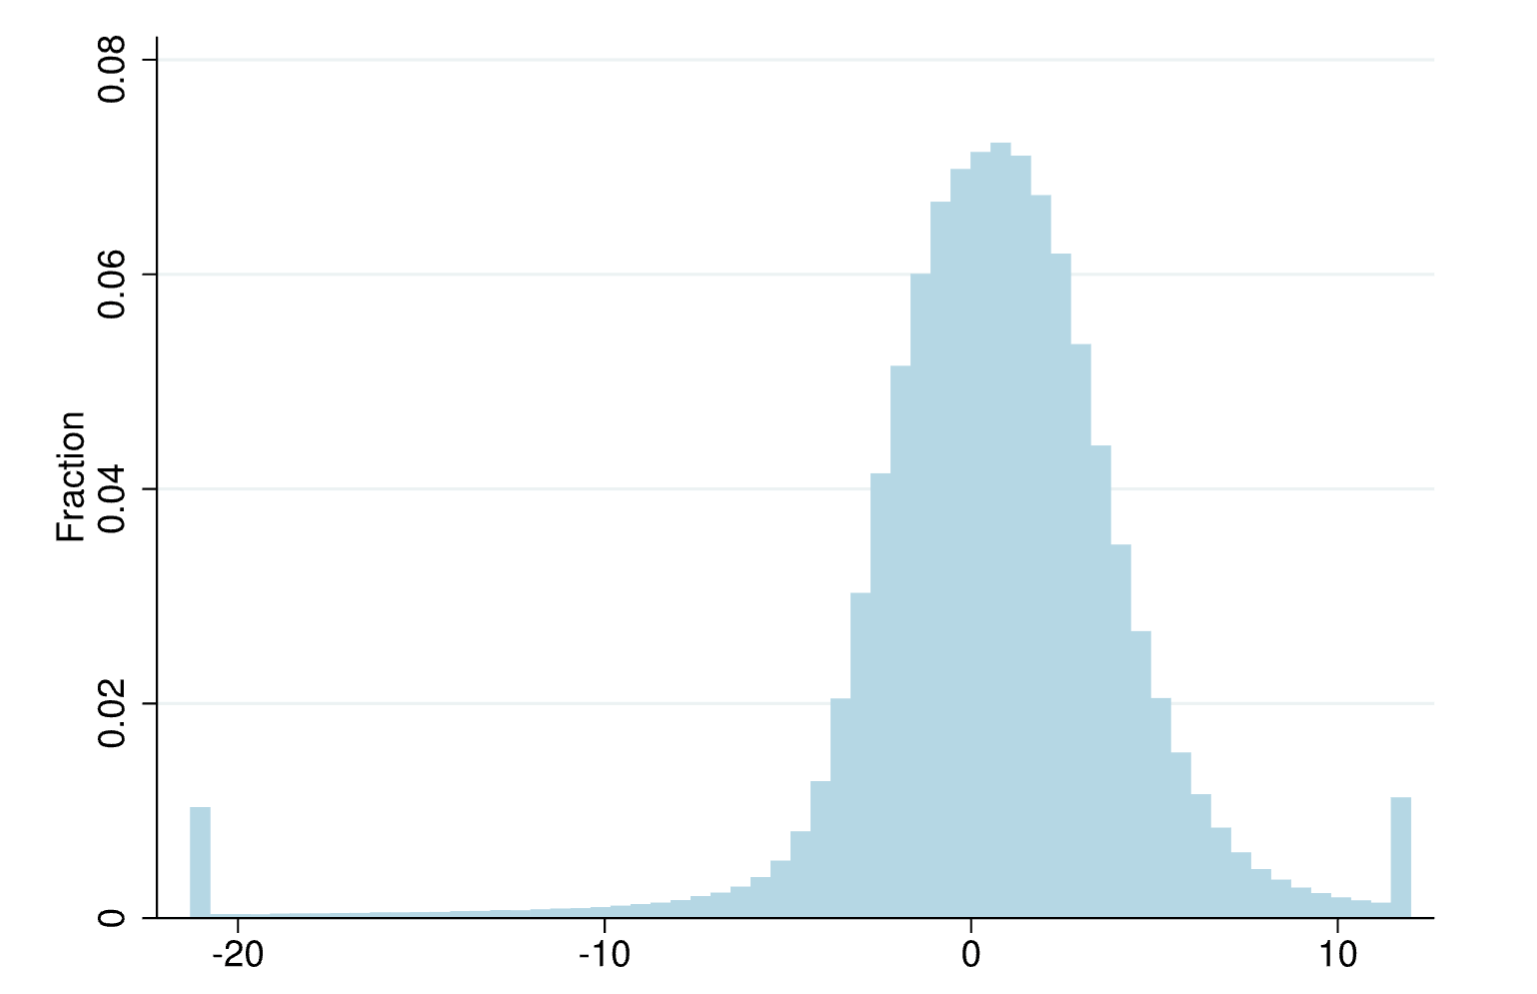
\includegraphics[width=\textwidth]{Figures/Fagereng2020Fig8.png}
    \captionsetup{font=scriptsize}
    \caption{Distribution of fixed effects in the return to net worth from \cite{aflgdmlp20}.}
    \end{figure}
  \end{columns}

\end{frame}
%%%%%%%%%%%%%%%%

\section{Model}
\subsection{Households}

\small
\begin{frame}{Labor income process}

\begin{itemize}
\item Household income: $$y_t = p_t \xi_t W_t$$
\item Permanent component: $$p_t = p_{t-1} \psi_t$$
\item Transitory component: $$\xi_t =
    \begin{cases}
       \mu & \text{with probability $\mho$} \\
      (1-\tau_t) \ell \theta_t & \text{with probability $1-\mho$}
   \end{cases}$$
\end{itemize}
%\vspace{1.5mm}

\end{frame}
%%%%%%%%%%%%%%%%%
%Put equations for permanent and transitory income%

\footnotesize
\begin{frame}{(Normalized) Optimization problem}

Choose consumption profile $\{c_{t_n}\}_{n=0}^{\infty}$ that maximizes
 \begin{eqnarray*}
  v(m_t) &=& \max_{c_t} u(c_t(m_t)) + \beta \cancel{D} \mathbb{E}_{t}[\psi_{t+1}^{1-\rho}v(m_{t+1})] \\
  &\text{s.t.}& \\
  \underbrace{a_t}_{\text{assets today}} &=& m_t - c_t(m_t), \\
  \underbrace{k_{t+1}}_{\text{capital tomorrow}} &=& \frac{a_t}{\cancel{D}\psi_{t+1}}, \\
  \underbrace{m_{t+1}}_{\text{market resources tomorrow}} &=& \underbrace{(1 - \delta + \textcolor{red}{r_t})k_{t+1}}_{\text{bank balances}} + \underbrace{\xi_{t+1}}_{\text{perm. inc. unit scaled by trans. shock}}. \\
 \end{eqnarray*}

 

%Production function $$Y = Z K^{\alpha} (\ell L)^{1-\alpha}$$

\end{frame}
%%%%%%%%%%%%%%%%%

\subsection{Simulation}

\begin{frame}{Calibration}
\vfill
\begin{table}
  \centering
  %\scriptsize  % or \tiny, \footnotesize as needed
  \hypertarget{calibPY}{}
\begin{table}[ht]
  \centering
  \resizebox{0.7\textwidth}{!}{
    \begin{tabular}{cccc}
        \toprule
        Description & Parameter & Value \\
        \midrule
        Time discount factor & $\beta$ & 0.99$^4$ \\
        CRRA & $\rho$ & 1  \\
        Capital share & $\alpha$ & 0.36  \\
        Depreciation rate & $\delta$ & 0.025  \\
        Time worked per employee & $\ell$ & 1/.09  \\
        Wage rate & $W$ & 2.37  \\
        Unempl. insurance payment & $\mu$ & 0.15 \\
        Probability of survival & $\cancel{D}$ & (1 - 0.00625)$^4$  \\
        Std. dev of $\log \theta_{t,i}$ & $\sigma^{2}_{\theta}$ & 0.010 x 4 x $\sqrt{4}$  \\
        Std. dev of $\log \psi_{t,i}$ & $\sigma^{2}_{\psi}$ & 0.010 x 4/11 x $\sqrt{4}$ \\
        Unemployment rate & $\mho$ & 0.07  \\
        \bottomrule
    \end{tabular}}
    \caption{Parameter values (annual frequency) for the perpetual youth model.}
    \label{tab:calib1}
\end{table}


\end{table}
\vfill
\end{frame}


%%%%%%%%%%%%%%%%



\begin{frame}{Estimation procedure}


Simulated method of moments (SMM) estimation for $R$ using 2004 SCF wealth data.


  \begin{enumerate}
  \item No ex-ante heterogeneity: $R$\textit{-point} model
    \par Estimate a common rate of return:

    \par  \say{Center} so the model  matches the capital-to-output ratio $(\frac{K}{Y} = 3)$.
  \vspace{2.5mm}

  \item Ex-ante heterogeneity: $R$\textit{-dist} model
    \par Estimate  a \textbf{Uniform distribution} of returns:

    \par \say{Center} and \say{spread} so the model matches SCF Lorenz targets, given $\frac{K}{Y}$.
  \end{enumerate}

   \vspace{2.5mm}
  \centering
  \small
  \begin{tabular}{|c|c|}
\hline
Net worth percentile & Cumulative net worth \\
\hline
20th & -.18\%  \\
40th &  .95\% \\
60th &  5.3\% \\
80th &  17.09\% \\
\hline
\end{tabular}


\end{frame}

%%%%%%%%%%%%%%%%%

\section{Results}

\begin{frame}{How good is the fit?}

   \begin{columns}
    \column{0.5\textwidth}
    \centering
    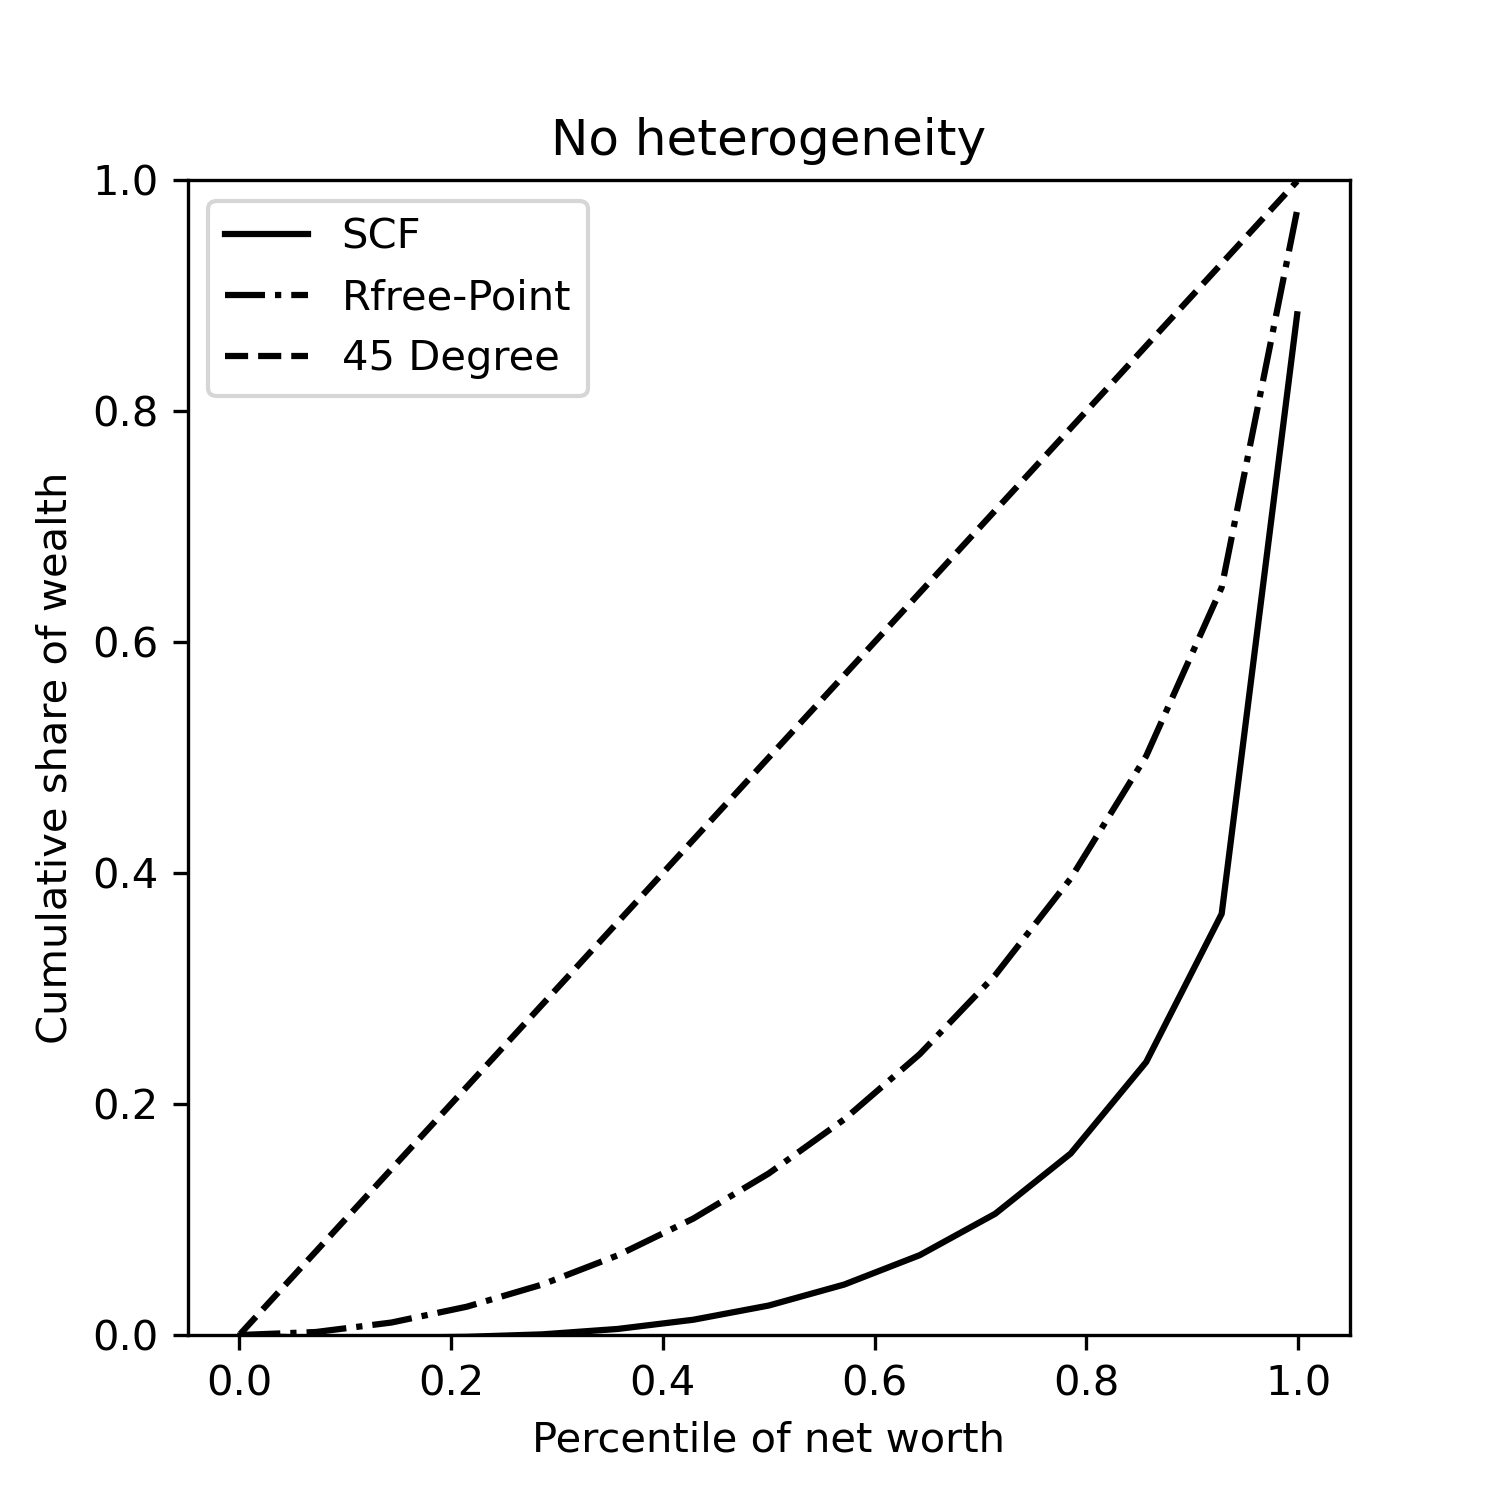
\includegraphics[width=\textwidth]{Figures/PYrrPointNetWorthPlot.png}

    \column{0.5\textwidth}
    \centering
    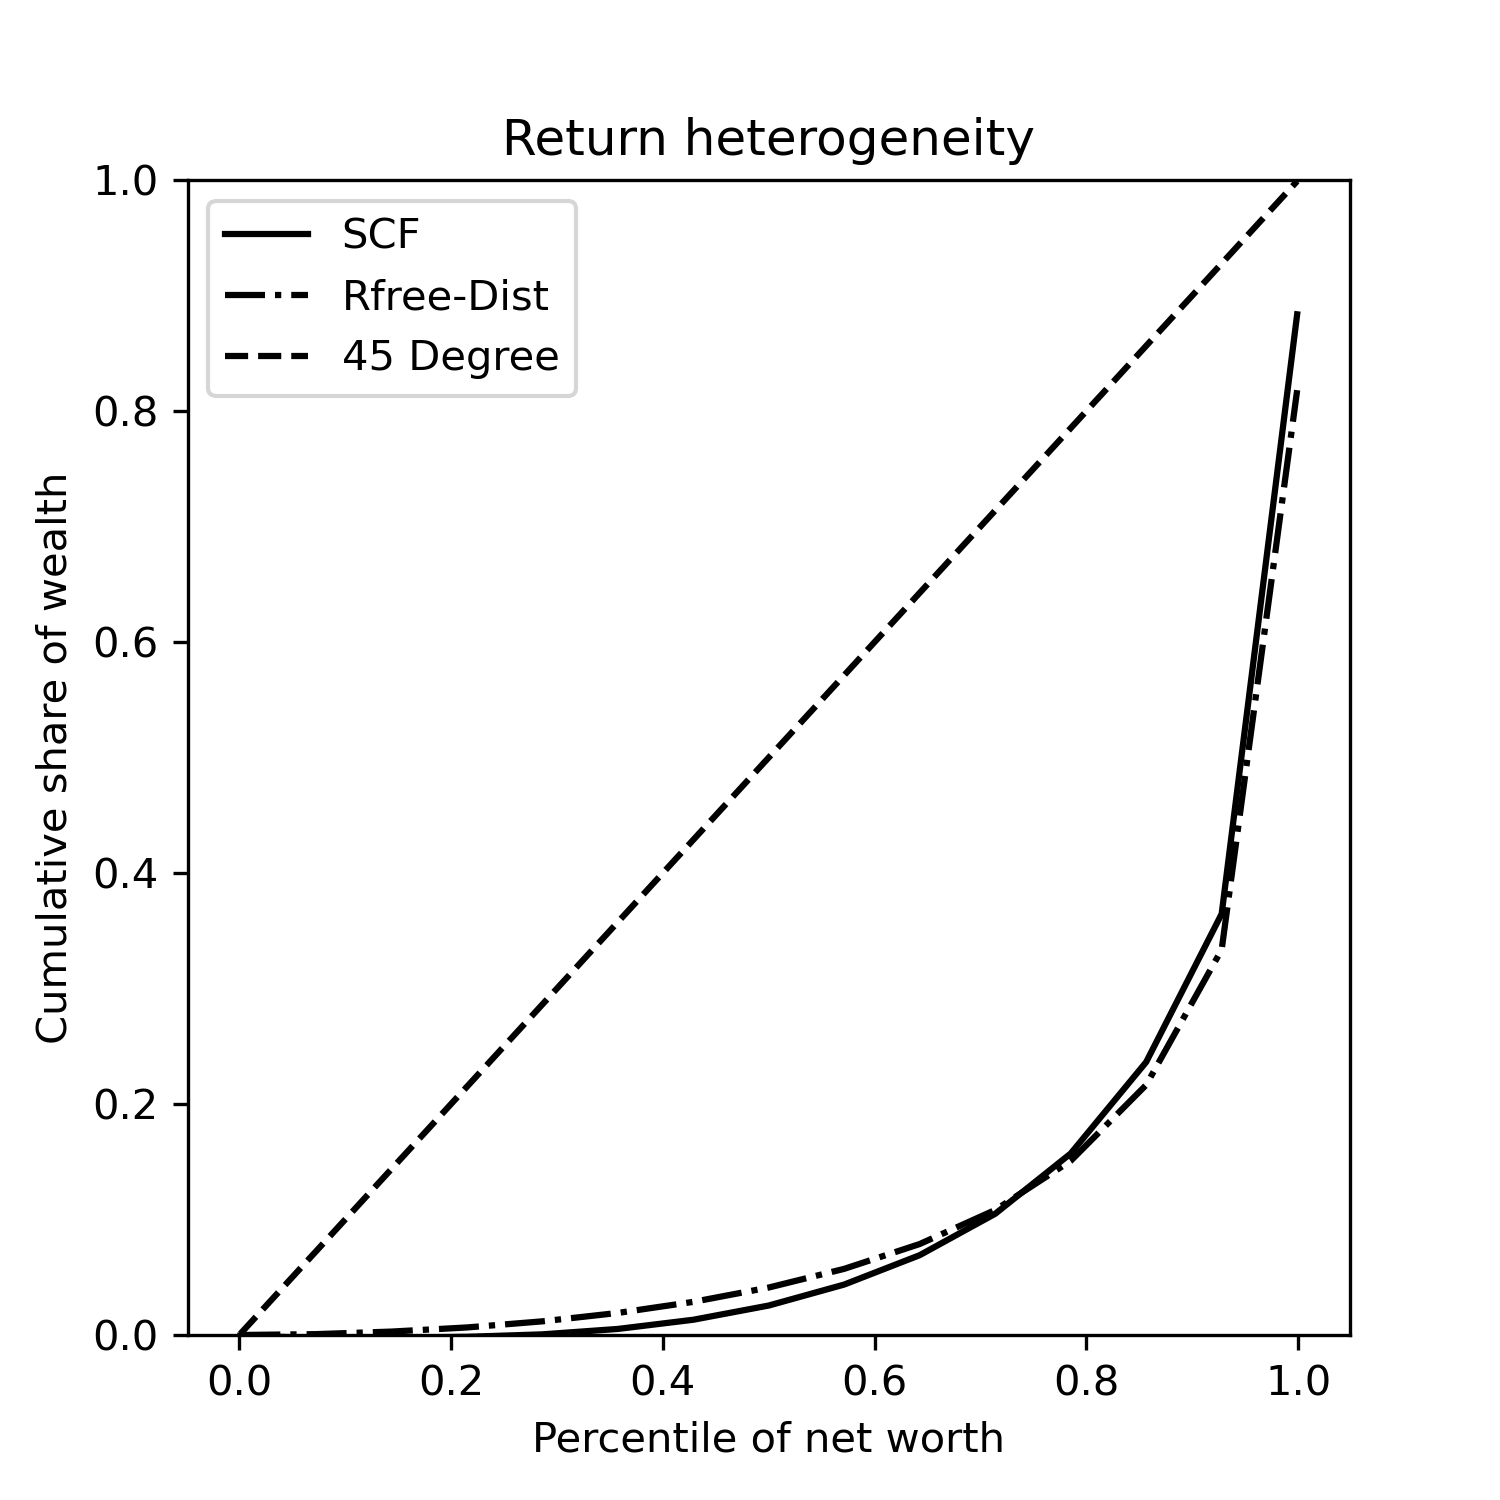
\includegraphics[width=\textwidth]{Figures/PYrrDistNetWorthPlot.png}

  \end{columns}

\end{frame}

%%%%%%%%%%%%%%%

\begin{frame}{Lifecycle version of the model}
\begin{itemize}
\item Education cohort $e \in \{D, HS, C\}$
\item Initial wealth-to-income $k_0$ and income $p_0$ levels
\item Education-age dependent mortality rates
\par \parencite{Brown2007}
\item Modified labor income uncertainty $y_t = \xi_t \psi_t \overline{\psi}_{es} p_{t-1}$
\par \parencite{Cagetti2003}
\end{itemize}
\end{frame}
%%%%%%%%%%%%%%%

\begin{frame}{Calibration}
\vfill
\begin{table}
  \centering
  \scriptsize 
  \hypertarget{calibLC}{}
\begin{table}[ht]
  \centering
  \resizebox{0.6\textwidth}{!}{
    \begin{tabular}{ccc}
        \toprule
        Description & Parameter & Value  \\
        \midrule
        Population growth rate & $N$ & 0.0025  \\
        Technological growth rate & $\Gamma$ & 0.0037  \\
        Rate of high school dropouts & $\theta_D $ & 0.11  \\
        Rate of high school graduates & $\theta_{HS} $ & 0.55  \\
        Rate of college graduates & $\theta_C $ & 0.34  \\
        Labor income tax rate & $\tau$ & 0.0942  \\
        \bottomrule
    \end{tabular}}
    \caption{Parameter values (annual frequency) for the lifecycle model.}
    \label{tab:calib2}
\end{table}


\end{table}
\vfill
\end{frame}

%%%%%%%%%%%%%%%%%%


\begin{frame}{How good is the fit?}
 \begin{columns}
    \column{0.5\textwidth}
    \centering
    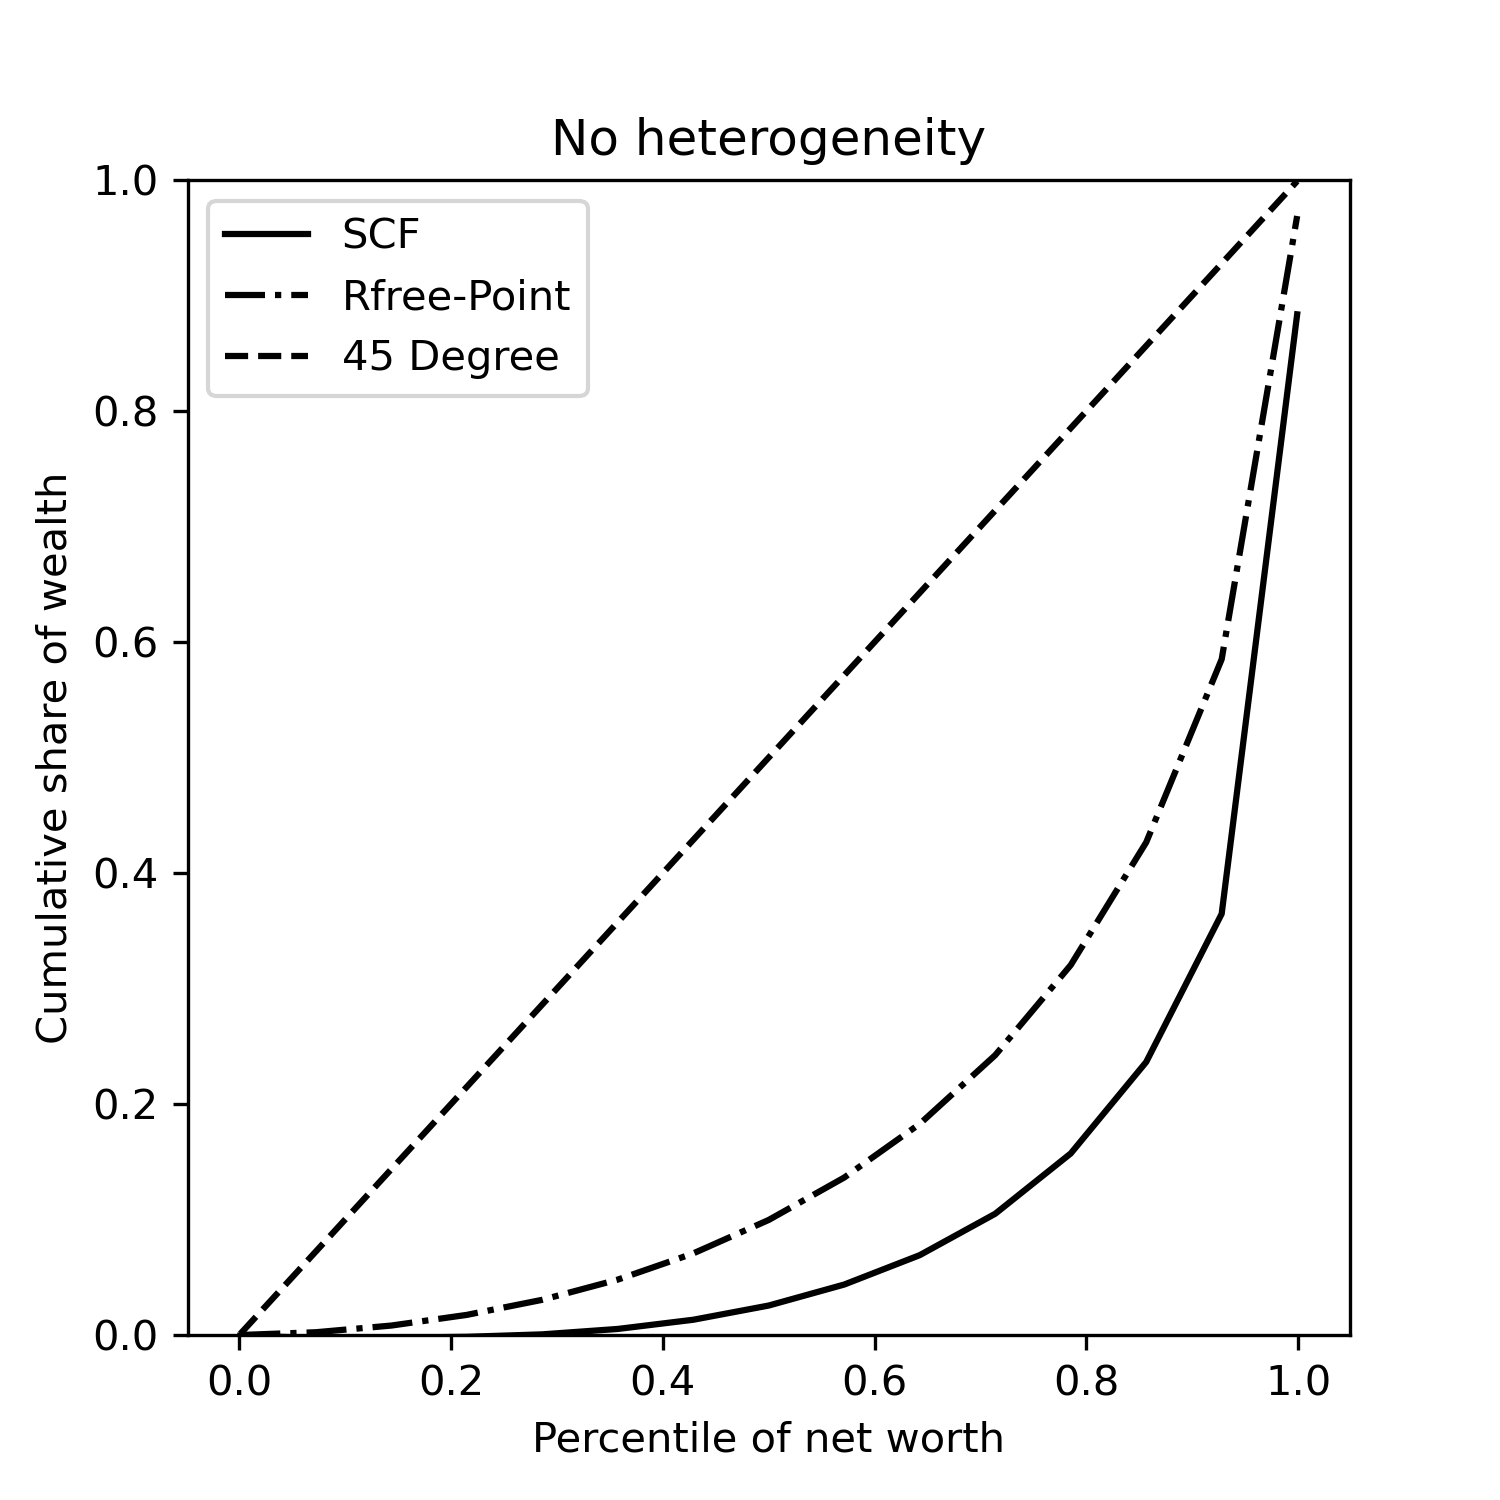
\includegraphics[width=\textwidth]{Figures/LCrrPointNetWorthPlot.png}

    \column{0.5\textwidth}
    \centering
    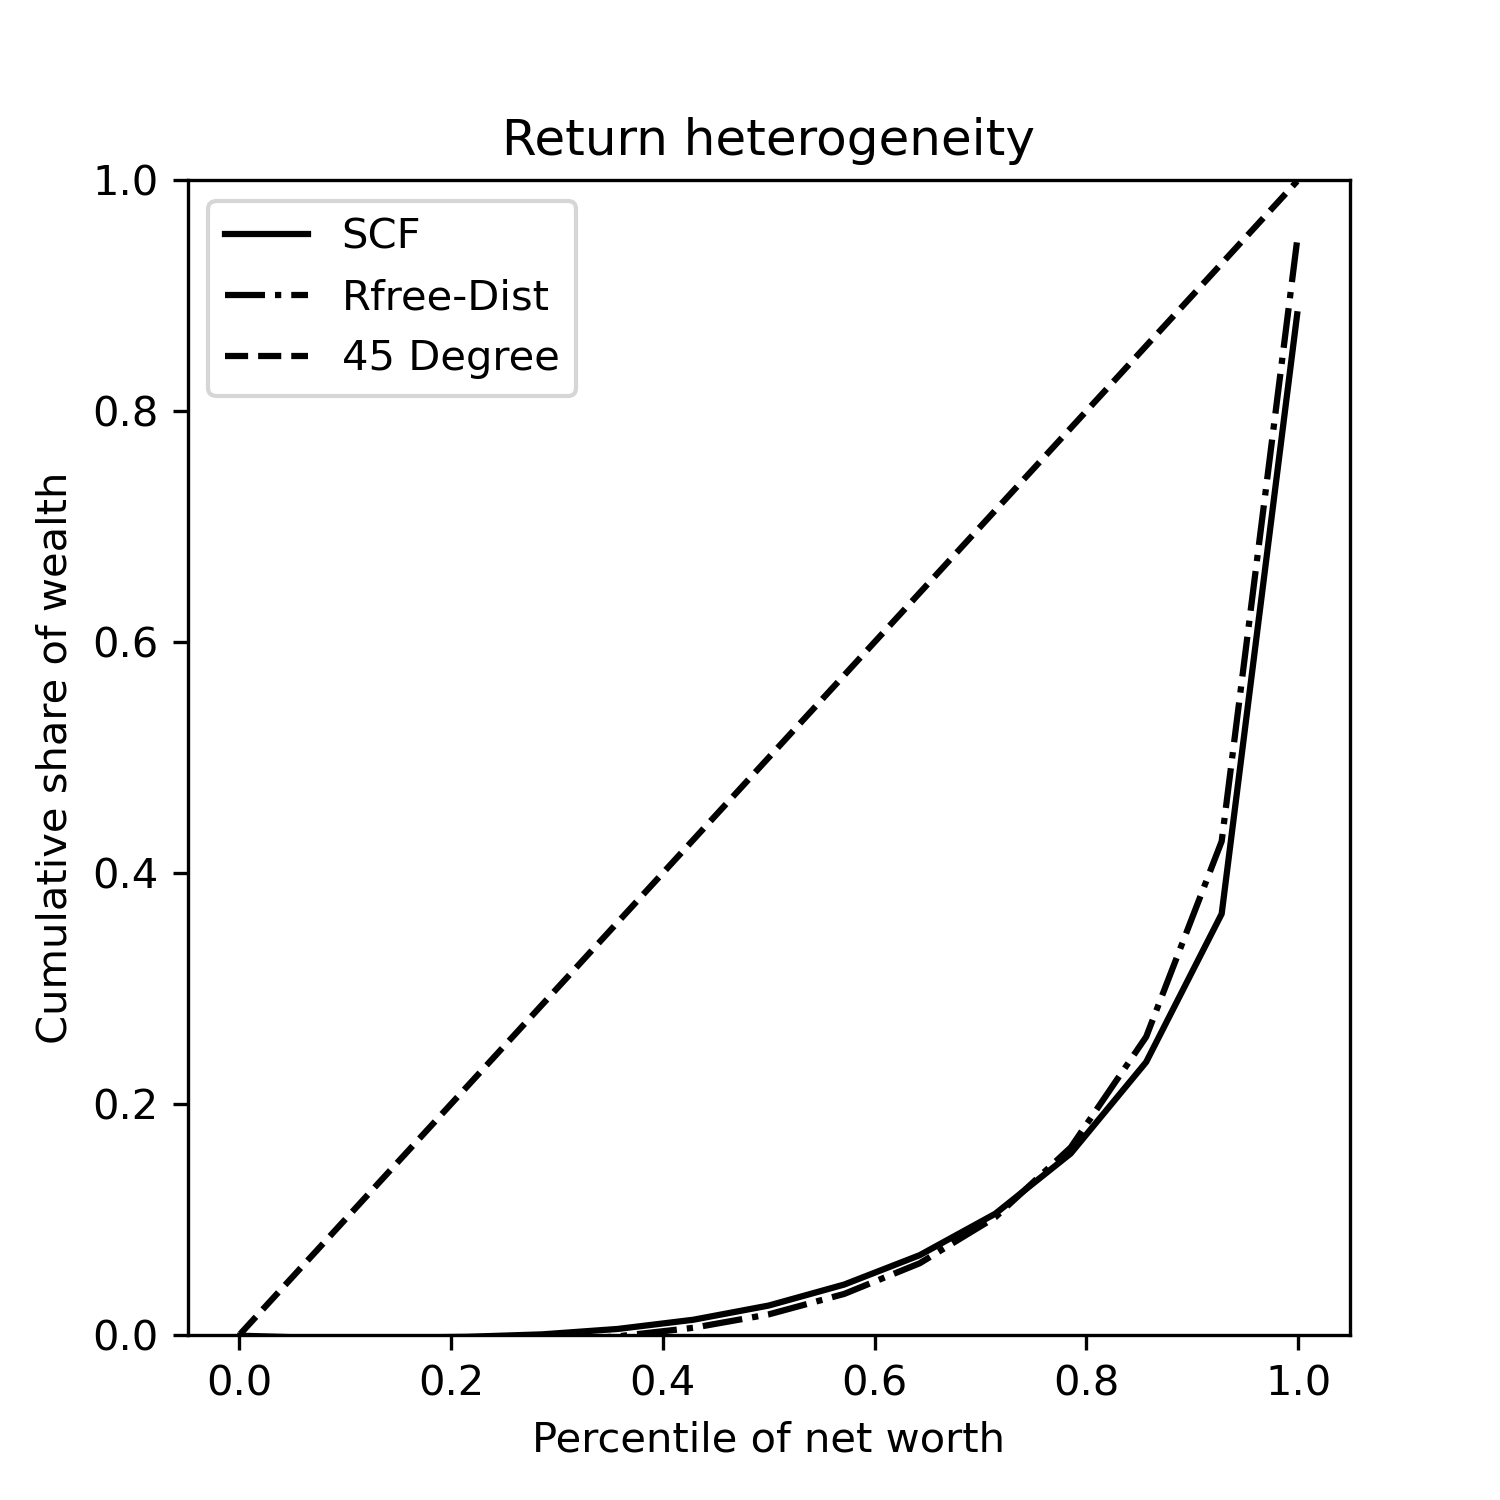
\includegraphics[width=\textwidth]{Figures/LCrrDistNetWorthPlot.png}

  \end{columns}
\end{frame}

%%%%%%%%%%%%%%%%

\begin{frame}{Model performance: returns distribution}
\centering

\begin{flushleft}
\par Empirical values from \cite{aflgdmlp20}
\end{flushleft}
    \begin{tabular}{|c|c|c|}
\hline
& Mean & St. Dev \\
\hline
Net worth (after tax) & 0.0365 & 0.0781  \\
\hline
\end{tabular}

\begin{flushleft}
\par Values from the structural estimation (uniform distribution for $R$)
\end{flushleft}
    \begin{tabular}{|c|c|c|}
\hline
& Mean & St. Dev \\
\hline
PY-Point & 0.060 & 0.0  \\
PY-Dist & 0.021  &  0.011  \\
LC-Point & 0.040 & 0.0  \\
LC-Dist & 0.023  &  0.009  \\
\hline
\end{tabular}

\end{frame}
%%%%%%%%%%%%%%%%%%

\begin{frame}{Model performance: untargeted moments}
\centering
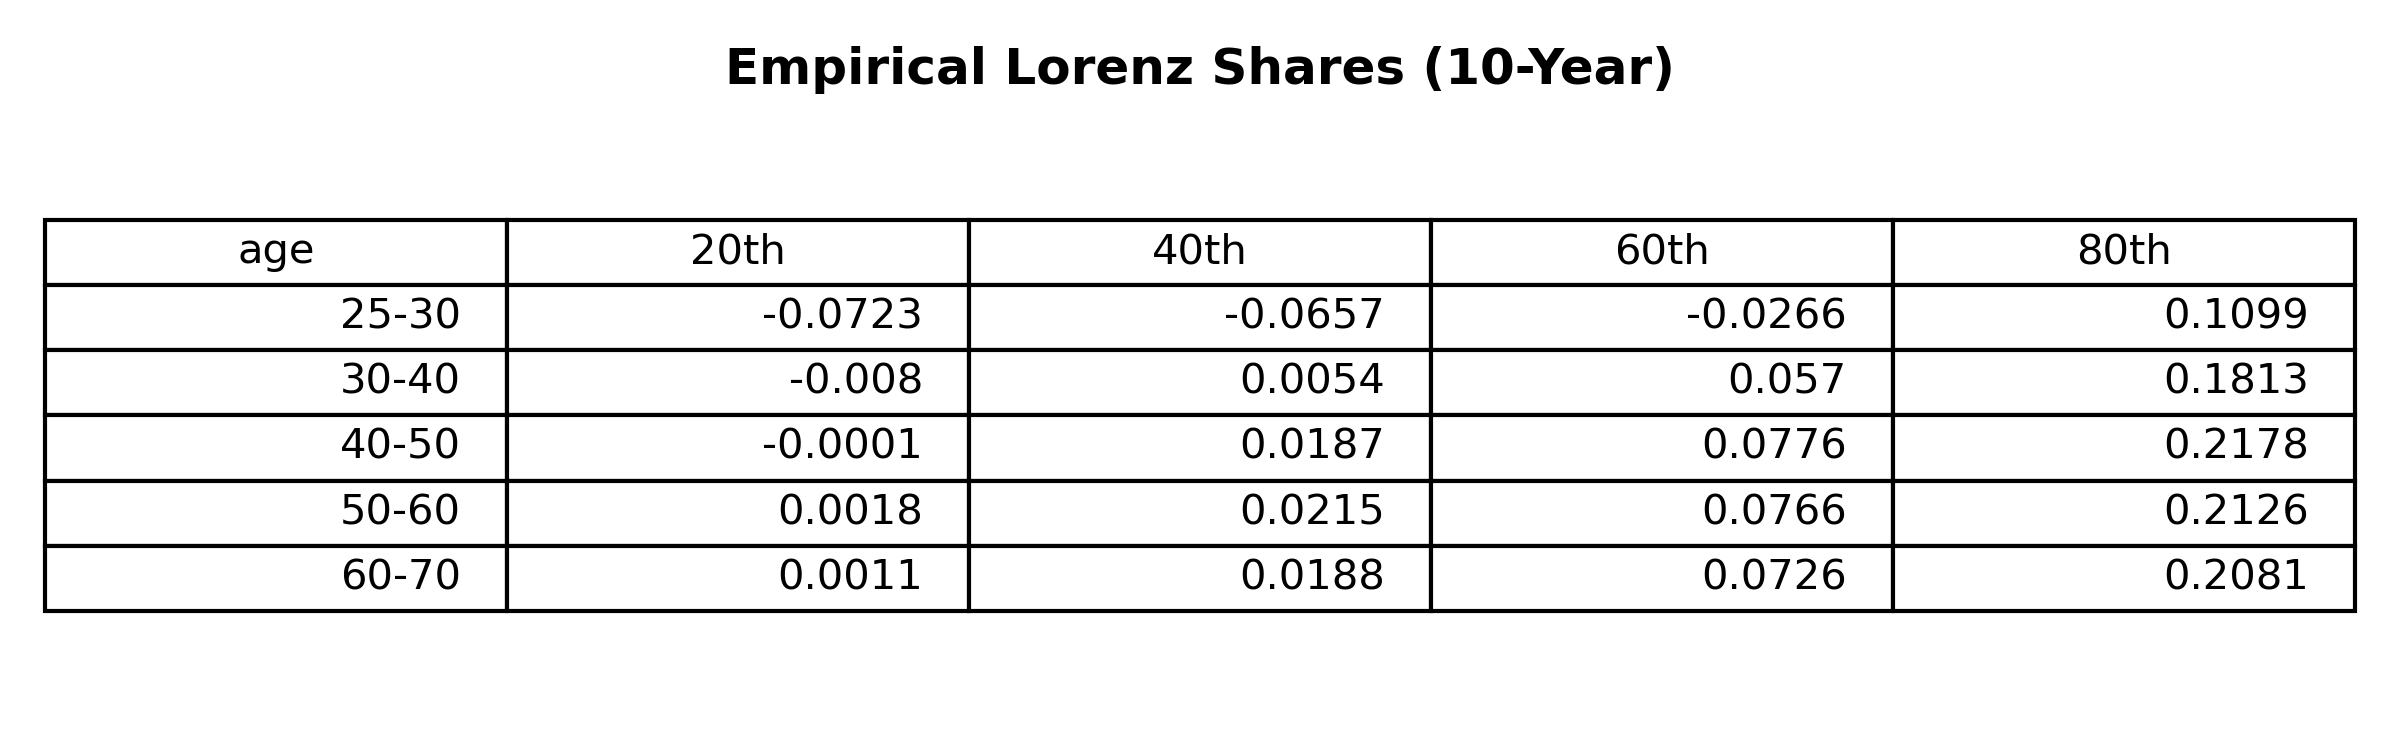
\includegraphics[width=0.8\textwidth]{Tables/Emp_Lorenz_10yr_LCrrDistNetWorth.png}

%\vspace{0.5cm} % vertical space between the two tables/images

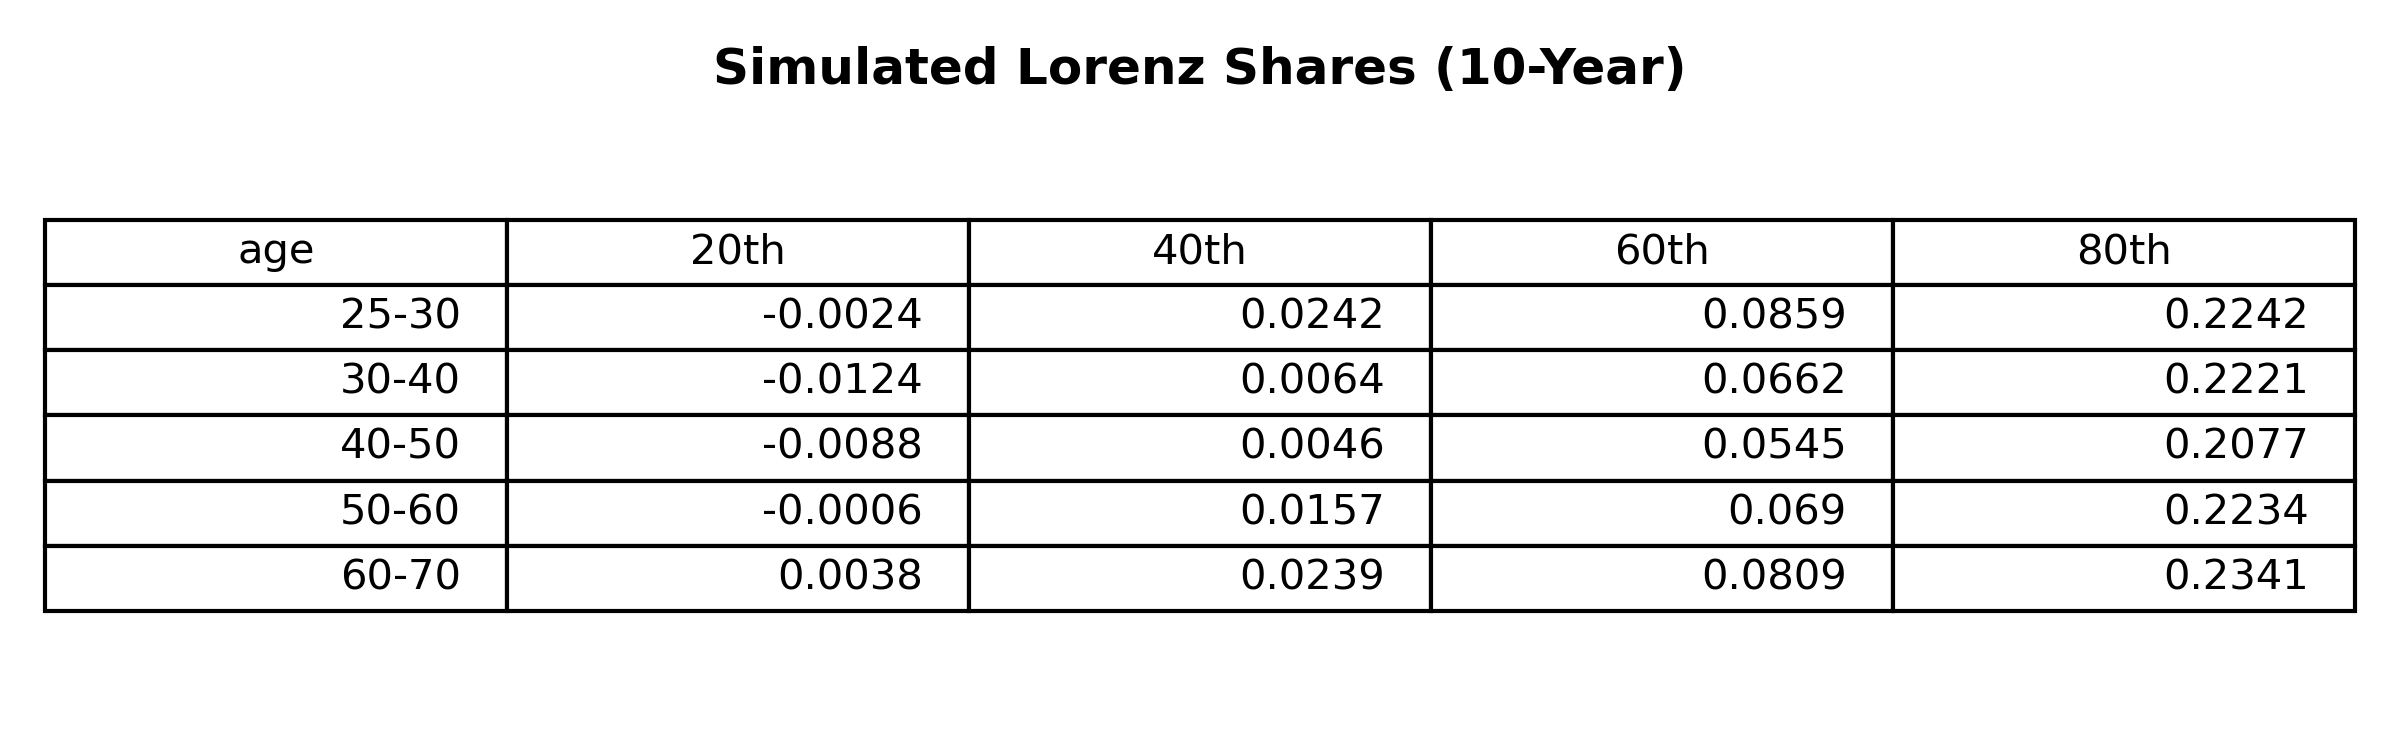
\includegraphics[width=0.8\textwidth]{Tables/Sim_Lorenz_10yr_LCrrDistNetWorth.png}

\end{frame}

%%%%%%%%%%%%%%%%%%

\subsection{Banks}
\begin{frame}{Potential sources of return heterogeneity}
  \begin{itemize}
  \item Entrpreneurship - \say{high levels of capital, low MPK}
  \item Financial literacy - closer, but generally aimed at risky assets
    \end{itemize}

    \vspace{2.5mm}
    Remember, there is het. returns even when holding only safe assets.  

     \vspace{2.5mm}
     \par Business Insider - \say{Average Bank Account Interest rates}
     \begin{itemize}
     \item \textit{On average, interest-bearing checking accounts earn $0.07\%$ APY.}
       \item However, many checking accounts exist whiuch offer up to 3.3\% APY.
  \end{itemize}

   \vspace{2.5mm}
     \par Is there a mechanism we can exploit?
  \end{frame}

  %%%%%%%%%%%%%%%%%%%%%%%%%%

\begin{frame}{Mechanism}

\begin{itemize}
    \item \say{Transmission channel of monetary policy} by  \cite{Drechsler2017}
      \begin{itemize}
      \item Sensitivity of bank deposits to market interest rate changes
      \end{itemize}
      \end{itemize}
  
 \begin{itemize}
  \item $\Delta$ in market rate $\rightarrow$ variation in $\Delta$ in deposits held at banks
    \begin{itemize}
  \item \cite{Sarkisyan2021} - globally integrated vs local banks
  \item \cite{dAvernas2024} - small vs large banks
    \end{itemize}
  \end{itemize}

  \vspace{2.5mm}
  $\implies$ variation in deposit rates offered across banks
  
\end{frame}

  %%%%%%%%%%%%%%%%%%%%%%%%%%%5
\begin{frame}[label=bankmodel]{A simple model of bank heterogeneity}

\par Let $R^m$ be the market rate of return, $R^d$ be the rate of return offered on deposits by a  bank, and $S(R^d, R^m)$ be the level of deposits held at a given bank.

 \vspace{2.5mm}
\par Banks solve:
\[
\max (R^m - R^d) \cdot S(R^d, R^m)
\]

\par subject to:
\[
S(R^d, R^m) = A \left( \frac{R^d}{R^m} \right)^{\varepsilon}
\]

\vspace{1em}
\hyperlink{epsilonslide}{\beamerbutton{Show interpretation of $\varepsilon$}}

\end{frame}

\begin{frame}[label=epsilonslide]{Interpreting the Elasticity Parameter $\varepsilon$}

\small
\par So $\varepsilon$ has a clear interpretation as the elasticity of deposits to changes in the market interest rate:

\[
-\varepsilon = \frac{\partial S(\cdot)}{\partial R^m} \cdot \frac{R^m}{S(\cdot)}
\]

\vspace{1em}
\hyperlink{bankmodel}{\beamerbutton{Back to model}}

\vspace{1em}
\hyperlink{focslide}{\beamerbutton{First order condition}}

\end{frame}

\begin{frame}[label=focslide]{Bank's optimal choice of  $R^d$}

\small
\par  The first order condition for the bank's optimization problem implies that:

\[
R^d  = \frac{\varepsilon}{1+ \varepsilon} R^m 
\]

\vspace{1em}
\hyperlink{bankmodel}{\beamerbutton{Back to model}}

\end{frame}
%%%%%%%%%%%%%%%%%%%%%%

\begin{frame}{Estimation procedure}

Simulated method of moments (SMM) estimation for $R$ using 2004 SCF wealth data.

%\vspace{5mm}
\begin{enumerate}
  \setcounter{enumi}{2} 
\item Implied distribution of elasticities $\epsilon$
  \par The solution to the bank's optimization problem implies
  \begin{align}
    \varepsilon = \frac{R^d}{R^m - R^d}
  \end{align}

  \par $\implies$ SMM procedure pins down a dist. of elasticites describing banking heterogeneity.
  \end{enumerate}

\end{frame}
%%%%%%%%%%%%%%%%%

\begin{frame}{Model performance: implied elasticites}

  \begin{center}
\begin{tabular}{|c|c|c|c|}
\hline
\multicolumn{2}{|c|}{PY} & \multicolumn{2}{|c|}{LC} \\
\hline
Estimated returns & Implied elasticities & Estimated returns & Implied elasticities \\
\hline
0.964 & 7.329 & 0.976 & 8.165 \\
0.983 & 8.755 & 0.991 & 9.564 \\
1.001 & 10.771 & 1.007 & 11.468 \\
1.021 & 13.837 & 1.023 & 14.208 \\
1.040 & 19.064 & 1.039 & 18.492 \\
1.060 & 29.974 & 1.055 & 26.136 \\
1.079 & 66.891 & 1.071 & 43.645 \\
\hline
\end{tabular}
\end{center}

\vspace{2.5mm}
\cite{Genay2004} - \say{A 1\% increase in the fed funds rate over four quarters is associated with a 2.96\% decline in the growth of core deposits at small banks and a 3.66\% decline at large banks.}

\end{frame}


%%%%%%%%%%%%%%%%%



\subsection{Concluding Remarks}


\begin{frame}{Work to be done}
  \begin{itemize}
\item Better empirical moments from \cite{aflgdmlp20} to compare results to
\item Implications of wealth tax vs capital income tax when het. returns are present \cite{Guvenen2023}
\end{itemize}
\end{frame}


%%%%%%%%%%%%%%%%%%%%%
%\begin{frame}{Work to be done}

 %      \begin{enumerate}
  %     \item Robustness checks
   %    \begin{itemize}
    %  \item Plausible parameter values for time preferences and risk aversion
   %   \item Different measures of wealth (liquid and/or financial)
   %   \end{itemize}
  %  \item More untargeted moments
   %   \begin{itemize}
     %   \item Wealth shares by education cohort
    %    \end{itemize}
   % \end{enumerate}

%\end{frame}
%%%%%%%%%%%%%%



\begin{frame}[allowframebreaks]{References}
  \printbibliography
\end{frame}

\end{document}




